\section{The Stack}
\label{sec:stack}

LLVM intermediate representation is written in static single assignment (SSA) form. This property states that each variable is assigned exactly once, with variables being split into versions, and every variable receiving its own definition. The motive behind SSA form is that it simplifies and improves the results of various compiler optimisations by more explicitly stating data dependencies. However, The Dalvik executable format is register-based, so we have no need for SSA form while generating code: variables are held in a fixed set of registers, and when a variable is written to we can no longer access the old value (nor do we need to).

To this end, we instead allocate mutable variables on the stack and use load and store instructions to access them. In LLVM, all memory accesses are explicit with load/store instructions. Every read of a value then becomes a load from the stack, and each update of a variable becomes a store to the stack. This paradigm introduces a problem; we now introduce a lot of stack traffic for simple and commonplace operations. This is evidently a major performance issue. The LLVM optimiser has a solution to this problem: the `mem2reg' pass. This optimisation promotes memory accesses to register variables and tidies up the loose ends. This is a high-performance optimisation that is used by major LLVM front-ends such as clang and llvm-gcc\footnotemark \footnotetext[1]{http://llvm.org/docs/tutorial/LangImpl7.html\#memory}. We rely on this optimisation pass to keep the generated code performing well.

Care must be taken while translating a Dalvik method into LLVM bytecode. If the code generator is too na\"{\i}ve in its instruction selection, difficulties can arise. Allocating a register variable on the stack as soon as the code generator comes across it leads to major problems, specifically when control-flow comes into play.

Let us now consider a simple example in which a problem might arise. Take the sample Java snippet:

\lstset{
	language=Java,
	basicstyle=\small,
	stringstyle=\ttfamily
}

\begin{lstlisting}[frame=single, numbers=left, numberstyle=\tiny, caption={Java control-flow example}, label=lst:java_br]
int x;
if (a < b)
    x = 0;
else
    x = 1;
return;
\end{lstlisting}

and its Dalvik translation:

\lstset{
	language=Assembly,
	basicstyle=\small,
	stringstyle=\ttfamily
}

\begin{lstlisting}[frame=single, numbers=left, numberstyle=\tiny, caption={Dalvik code for Listing \ref{lst:java_br}}, label=lst:dalvik_br]
if-ge a, b, 4
const x, 0
return void
const x, 1
goto 3
\end{lstlisting}

In Listing \ref{lst:dalvik_br}, the branch targets in the \verb|if-ge| and \verb|goto| instructions are absolute and refer to the line numbers at the left of the code frame. Additionally, this section of Dalvik bytecode might be represented by the control-flow graph (CFG) in Figure \ref{fig:cfg_dalvik}.

Looking at the example in Listing \ref{lst:dalvik_br}, we see the order of instructions that the code generation component will process. We are also able to see the basic blocks in which each instruction resides from Figure \ref{fig:cfg_dalvik}. After translating the branch instruction, we come across the instruction on line 2 of Listing \ref{lst:dalvik_br}: the store of the constant 0 to the variable \verb|x|. We are currently generating instructions from within the basic block on the left.

\begin{figure}[h!]
    \centering
    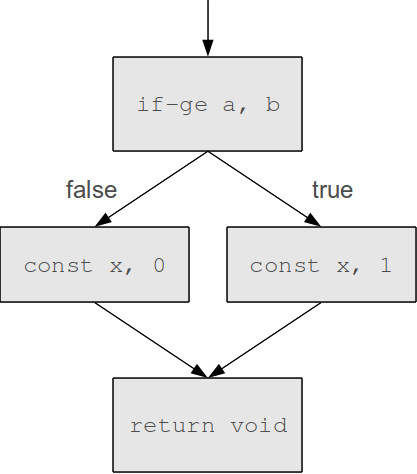
\includegraphics[width=0.5\textwidth]{images/cfg_dalvik.png}
    \caption{CFG representation of Listing \ref{lst:dalvik_br}}
    \label{fig:cfg_dalvik}
\end{figure}

Assuming that we have not seen the variable \verb|x| before, we create a new integer allocation on the stack in which we store the appropriate value. Generating code na\"{\i}vely, we have placed the allocation inside the basic block in which we reside. By the time that we come to the second store instruction, we have moved into the basic block on the right of Figure \ref{fig:cfg_dalvik}. The variable \verb|x| has been previously discovered and handled by the code generator, and so we do not need to create another allocation. We continue, store the value 1 into the variable, and complete the translation from Dalvik to LLVM bytecode. The CFG associated with this generated section of LLVM bytecode is detailed in Figure \ref{fig:cfg_llvm}.

\begin{figure}[h!]
    \centering
    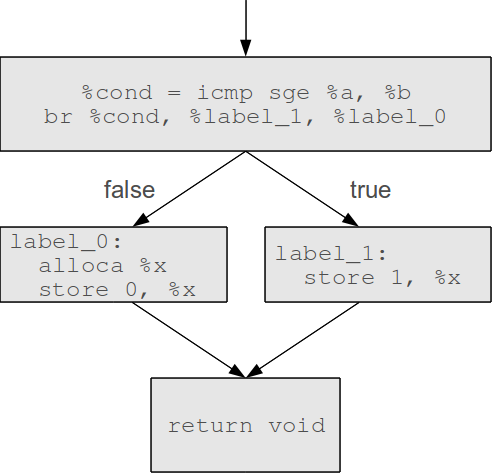
\includegraphics[width=0.5\textwidth]{images/cfg_llvm.png}
    \caption{CFG for the LLVM bytecode of Listing \ref{lst:dalvik_br}}
    \label{fig:cfg_llvm}
\end{figure}

However, there is a major problem with this resulting LLVM module. The allocation that we created in the first basic block does not dominate all of its uses. For example, if the condition on the branch instruction was true, i.e., \verb|a| was \textit{not} strictly less than \verb|b|, then the program would jump into the latter basic block - skipping the first entirely - and attempt to store a value to an as-of-yet unallocated variable \verb|x|. This is evidently a major error in the module, and the program would segmentation fault if run.

One solution to this pitfall is to create all allocations in a place where they dominate all subsequent instructions, i.e., they have function-wide scope. Therefore we introduce a new basic block to the start of every method, in which we carry out all stack allocations, in order to ensure that they have function-wide scope. We name this basic block \verb|allocas|, and it will feature in all subsequent LLVM bytecode listings. The unconditional branch from the allocation block to the first block of the method will be omitted, to avoid cluttering an example.

The corrected LLVM module of this example is shown in Figure \ref{fig:cfg_llvm2}, where the allocation of the variable \verb|x| is moved up to the dominator block at the beginning of the function. In this way we can guarantee that all load and store instructions to this variable are legal.


\begin{figure}[h!]
    \centering
    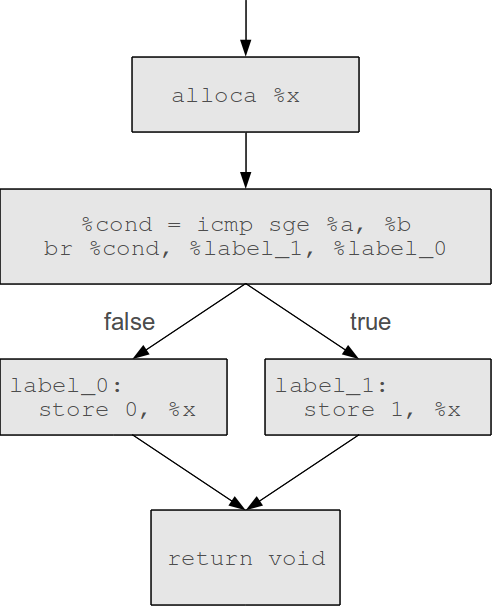
\includegraphics[width=0.5\textwidth]{images/cfg_llvm2.png}
    \caption{CFG for the corrected LLVM bytecode of Listing \ref{lst:dalvik_br}}
    \label{fig:cfg_llvm2}
\end{figure}

